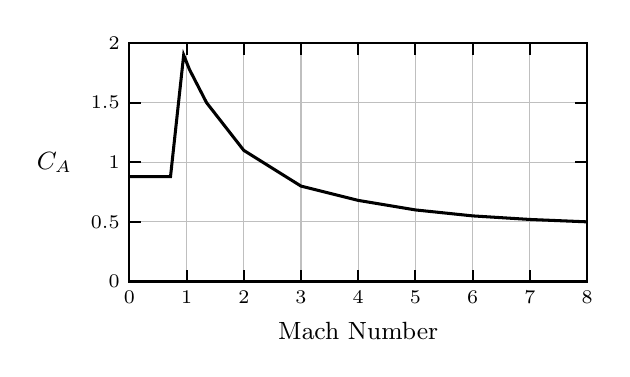
\begin{tikzpicture}
\begin{axis}[
  width=0.61\linewidth,
  height=0.38\linewidth,
  xmin=0,xmax=8,
  ymin=0,ymax=2,
  xtick={0,1,...,8},
  ytick={0,0.5,1,1.5,2},
  grid=major,
  axis line style={line width=0.8pt},
  tick style={black,line width=0.7pt},
  xlabel={Mach Number},
  ylabel={$C_A$},
  ylabel style={rotate=-90},
  label style={font=\small},
  tick label style={font=\scriptsize}
]
\addplot[black,line width=1.1pt] coordinates {
  (0,0.88) (0.72,0.88) (0.95,1.90) (1.05,1.78) (1.35,1.50)
  (2,1.10) (3,0.80) (4,0.68) (5,0.60) (6,0.55) (7,0.52) (8,0.50)
};
\end{axis}
\end{tikzpicture}
